\chapter{Spectral Analysis}
\label{chp:spectral_analysis}

This chapter is intended to give an overview of the spectral properties and limitations specific to multiplicative light field displays.
Spectral analysis is a crucial method for the quality assessment and it is the origin of a comprehensive understanding of 3D displays. 
A light field emitted by the display can be interpreted as a signal that is composed of sine waves with different amplitude, phase and frequency.
Section~\ref{sec:Definitions} introduces the Fourier transform, an operation that decomposes such a signal into the frequencies that produce it.
The spectral support, i.e. the range of frequencies the display is able to produce, is analyzed in section~\ref{sec:Spectral_Support_for_Display}. 

\section{Definitions}
\label{sec:Definitions}

The \textbf{Fourier transform} $\widehat{f}$ of an integrable function $f \colon \mathbb{R}^n \to \mathbb{C}$ is defined as 
\begin{equation}
	\widehat{f}(\xi) = \mathcal{F}(f)(\xi) \coloneqq \int_{\mathbb{R}^n} f(x) e^{-2 \pi \mathrm{i} x \cdot \xi} \, \mathrm{d}x
\end{equation}
for any $\xi \in \mathbb{R}^n$. 
According to the Fourier integral theorem, if both $f$ and $\widehat{f}$ are absolutely integrable and $f$ is continuous, then the inverse transform 
\begin{equation}
	f(x) = \mathcal{F}^{-1}(\widehat{f} \, )(x) \coloneqq \int_{\mathbb{R}^n} \widehat{f}(\xi) e^{2 \pi \mathrm{i} x \cdot \xi} \, \mathrm{d}\xi
\end{equation}
is well-defined.
The domain of $f$ is called the \textbf{spatial domain} and the domain of $\widehat{f}$ is referred to as the \textbf{frequency domain}.
An important property of the Fourier transform is that a convolution in the spatial domain becomes a multiplication in the frequency domain, or in other words, 
\begin{equation}\label{eq:convolution_theorem_1}
	\widehat{(f \ast g)}(\xi) = \widehat{f}(\xi) \cdot \widehat{g}(\xi)
\end{equation}
for integrable functions $f, g \colon \mathbb{R}^n \to \mathbb{C}$.
On the other hand, a multiplication in the spatial domain becomes a convolution in the frequency domain after applying the Fourier transform, that is
\begin{equation}\label{eq:convolution_theorem_2}
	\widehat{(f \cdot g)}(\xi) = (\widehat{f} \ast \widehat{g})(\xi).
\end{equation}
These two properties of the Fourier transform are known as the convolution theorem.
The Fourier transform and its inverse can also be discretized so that the convolution theorem still holds.
Hence, for the following analysis it is immaterial which form of the Fourier transform is used.

\section{Spectral Support of Light Fields}
\label{sec:Spectral_Support_for_Light_Field}

Consider a scene with a bounded depth range between $Z_{\text{min}}$ and $Z_{\text{max}}$.
The two objects at the boundaries are shown in figure~\ref{fig:two_objects}, with the virtual image $s$ plane between them.
The consequent 2D light field $L(u, s)$ (or EPI) is depicted in figure~\ref{fig:epi_two_objects}.
From equation~\ref{eq:disparity_for_two_plane_parameterization} it follows that objects appear in the EPI with a slope $\frac{\textrm{d}u}{\textrm{d}s} = \frac{z - Z_u}{z - Z_s}$.
Substituting $z$ with $Z_\text{min}$ and $Z_\text{max}$ gives the slopes for the red and blue objects at the boundary, defining the range of slopes in the EPI for objects between the two.

\begin{figure}[tb]
	\begin{subfigure}{0.5\textwidth}
		\centering
		\documentclass{standalone}
\usepackage{tikz}
\usepackage{pgfplots}

\tikzset{align at bottom/.style={baseline=(current bounding box.south)}}

\begin{document} 
	\begin{tikzpicture}[scale = 0.27]
	
		\draw[->] (-5, 0) -- (5, 0) node[right] {$s$};
		\draw[<-] (-5, -5) -- (-5, 5) node[above] {$z$};
	
		\begin{scope}
			\clip (-5, -5) rectangle (5, 5);
			\draw[scale = 1, smooth, domain = -10 : 10, variable = \x, black, dashed] plot ({\x}, {3});
			\draw[scale = 1, smooth, domain = -10 : 10, variable = \x, black, dashed] plot ({\x}, {-2});
		\end{scope}
		
		\node[left] at (-5, 3) {$Z_\textrm{min}$};
		\node[left] at (-5, -2) {$Z_\textrm{max}$};
		
		\draw[ultra thick, blue] (0, 3) -- (2, 3);
		\draw[ultra thick, red] (-3, -2) -- (0, -2);
		
		% Phantom node for alignment
		\node[right, opacity = 0] at (-5, -5) {$s$};
		
	\end{tikzpicture}
\end{document}
		\caption{}
		\label{fig:two_objects}
		\vspace{0.5cm}
		\documentclass{standalone}
\usepackage{tikz}
\usepackage{pgfplots}

\tikzset{align at bottom/.style={baseline=(current bounding box.south)}}

\begin{document}
	\begin{tikzpicture}[scale = 0.35]
	
		\begin{scope}
			\clip (-5, -5) rectangle (5, 5);
			%\node[anchor = center, inner sep = 0, opacity = 0.4] at (0, 0) {\includegraphics[width = 5cm]{../Figures/spectral_support/fft_red_and_blue.png}};
		\end{scope}
		
		\draw[->] (-5, 0) -- (5, 0) node[right] {$\xi_s$};
		\draw[->] (0, -5) -- (0, 5) node[above] {$\xi_u$};
		
		% Invisible dummy node for symmetric alignment with caption
		\node[left, opacity = 0] at (-5, 0) {$\xi_s$};
		
		\begin{scope}
			\clip (-5, -5) rectangle (5, 5);
			\draw[scale=1, smooth, domain = -10 : 10, variable = \x, blue] plot ({\x},{ -1 / (- 7 / 3) * \x});
			\draw[scale=1, smooth, domain = -10 : 10, variable = \x, red] plot ({\x},{ -1 / (12 / 2) * \x});
		\end{scope}
		
	\end{tikzpicture}
\end{document}
		\caption{}
		\label{fig:epi_fourier_transform_1}
	\end{subfigure}
	\begin{subfigure}{0.5\textwidth}
		\centering
		\documentclass{standalone}
\usepackage{tikz}
\usepackage{pgfplots}

\tikzset{align at bottom/.style={baseline=(current bounding box.south)}}

\begin{document} 
	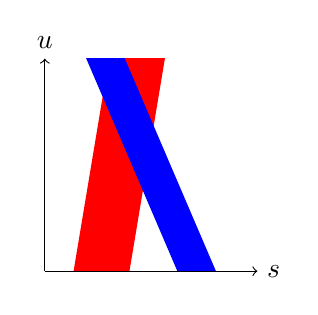
\begin{tikzpicture}[scale = 0.27]
	
		\begin{scope}
			\clip (-5, -5) rectangle (5, 5);
			\draw[scale = 1, smooth, variable = \x, red, line width = 0.7cm] plot ({\x}, { 12 / 2 * (\x + 1.5)});
			\draw[scale = 1, smooth, variable = \x, blue, line width = 0.45cm] plot ({\x}, { -7 / 3 * \x});
		\end{scope}
		
		\draw[->] (-5, -5) -- (5, -5) node[right] {$s$};
		\draw[->] (-5, -5) -- (-5, 5) node[above] {$u$};
		
	\end{tikzpicture}
\end{document}
		\caption{}
		\label{fig:epi_two_objects}
		\vspace{0.5cm}
%		\includegraphics[height = 3cm]{../Figures/spectral_support/fft_red_and_blue.png}
		\documentclass{standalone}
\usepackage{tikz}
\usepackage{pgfplots}

\tikzset{align at bottom/.style={baseline=(current bounding box.south)}}

\begin{document}
	\begin{tikzpicture}[scale = 0.27]
	
		\begin{scope}
			\clip (-5, -5) rectangle (5, 5);
%			\clip (-4.5, -4.5) rectangle (4.5, 4.5);
			\node[anchor = center, inner sep = 0, opacity = 1] at (0, 0) {\includegraphics[width = 5cm]{figures/spectral_support/fft_red_and_blue.png}};
		\end{scope}
		
		\begin{scope}
			\draw[->, opacity = 1] (-5, 0) -- (5, 0) node[right, opacity = 1] {$\xi_s$};
			\draw[->, opacity = 1] (0, -5) -- (0, 5) node[above, opacity = 1] {$\xi_u$};
		\end{scope}
		
		% Invisible dummy node for symmetric alignment with caption
		\node[left, opacity = 0] at (-5, 0) {$\xi_s$};
		
	\end{tikzpicture}
\end{document}
		\caption{}
		\label{fig:epi_fourier_transform_2}
	\end{subfigure}
	\caption[Spectral analysis for light fields with bounded depth range]
			{(a) Two objects (red and blue) placed at the bounds of the depth range. 
			 (b) The EPI representing the 2D light field of the scene.
			 (c) Fourier transform of the EPI. 
				 The red and blue line mark the bounds for the spectral support.
			 (d) Discrete Fourier transform of the EPI. 
				 Absolute values (magnitude response) are presented with colors on a logarithmic scale.
				 Blue indicates small magnitude and red color indicates high magnitude.}
	\label{fig:spectral_analysis_for_light_field}
\end{figure}

Applying the Fourier transform to the continuous light field reveals that the frequency response is non-zero on lines $\frac{\textrm{d}s}{\textrm{d}u} \xi_s + \xi_u = 0$. 
Again, for the scene with bounded depth range, this yields two lines representing the limits of the spectral support as shown in figure~\ref{fig:epi_fourier_transform_1}.
Objects between the red and blue ones will also have a frequency response within the fan spanned by the two lines.
Therefore, the region of support for a continuous light field with bounded depth range can be defined in the following way.
\begin{equation}\label{eq:region_of_support_for_light_field}
	\mathcal{S}(\xi_u, \xi_s) \coloneqq 
	    \begin{dcases*}
		    1, 			& if $Z_\text{min} \leq \dfrac{Z_u \xi_u + Z_s \xi_s}{\xi_u + \xi_s} \leq Z_\text{max}$ \\
		    0,			& otherwise $\vphantom{\dfrac{0}{0}}$ 
	    \end{dcases*}
\end{equation}
A similar expression follows for the 4D light field, defining a 4D hyperfan for the region of support as derived by~\cite{LinearVolumetricFocus}.
Note that occlusions as well as specular reflections are not incorporated in the above expression.
These effects introduce additional discontinuities in the EPI that result in a high frequency response possibly outside the fan defined in equation~\ref{eq:region_of_support_for_light_field}.

In the case of sampled light fields, aliasing can occur due to a small sampling rate in either angular- or spatial direction.
\cite{PlenopticSampling} analytically derived the minimum sampling rate required for alias-free light field rendering and proposed a reconstruction filter from known depth boundaries.
The region of support $\mathcal{S}(\xi_u, \xi_s)$ can also be thought of an ideal filter.
As equation~\ref{eq:convolution_theorem_1} shows, multiplying $\mathcal{S}(\xi_u, \xi_s)$ in the frequency domain is equivalent to a convolution in the spatial domain.

\section{Spectral Support of Layered 3D Displays}
\label{sec:Spectral_Support_for_Display}

With light field displays, it is of course desirable to achieve the same spectral coverage for the emitted light field as for the original.
Again, the analysis starts with the assumption of a continuous light field and an attenuator with $N$ continuously varying layers.
Each layer by itself creates a light field, and since the layer is at constant depth, the frequency response is non-zero along a slanted line as demonstrated before.
Let $L_1, \dots , L_N$ denote the constant depth light fields per layer and let's assume all are parameterized with respect to the same $(u, v)$- and \mbox{$(s, t)$-plane}.
The light field produced by all layers together is $L^\prime = L_0 \cdot L_1 \cdots L_N$, where $L_0$ is the uniform illumination from the backlight.
This directly follows from equation~\ref{eq:transmittance_layers}.
With the multiplication theorem from equation~\ref{eq:convolution_theorem_2}, the Fourier transform of $L^\prime$ can be expressed as
\begin{equation}\label{eq:convolution_of_layers}
	\widehat{L^\prime}(\xi) = (\widehat{L_0} \ast \widehat{L_1} \ast \cdots \ast \widehat{L_N}) (\xi), 
\end{equation}
where $\xi = (\xi_u, \xi_v, \xi_s, \xi_t)$, or $\xi = (\xi_u, \xi_s)$ for the two dimensional case.
For the case of discretely sampled layers, the frequency support of the individual layer will be limited by its spatial cutoff frequency, that is the highest frequency it can produce with a given pixel size $p$.
A signal with a period smaller than two pixels can not be reproduced by the layer's pixel grid and thus, the spatial cutoff frequency is defined as $\xi_0 = \frac{1}{2p}$ cycles/m.
\begin{figure}[tb]
	\begin{subfigure}[b]{.32\textwidth}
		\centering
		\documentclass{standalone}
\usepackage{tikz}
\usetikzlibrary{intersections}

\tikzset{align at bottom/.style={baseline=(current bounding box.south)}}

\begin{document}
	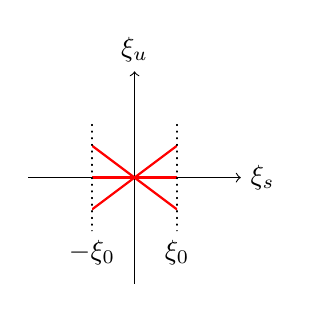
\begin{tikzpicture}[scale = 0.27]
	
		\draw[->] (-5, 0) -- (5, 0);
		\draw[->] (0, -5) -- (0, 5);
		\node[right] at (5, 0) {$\xi_s$};
		\node[above] at (0, 5) {$\xi_u$};
		
		%\draw[draw = black, fill = gray, fill opacity = 0.2, draw opacity = 0.5, name path = support_cut_off] (-4, 0) -- (-1.5, 3) -- (1.5, 3) -- (4, 0) -- (1.5, -3) -- (-1.5, -3) -- cycle;
		
		\begin{scope}
		
			\clip (-2, -2) rectangle (2, 2);
			
			\draw[red, thick, cap = round] (-2, 1.5) -- (2, -1.5);
			\draw[red, thick, cap = round] (-2, 0) -- (2, 0);
			\draw[red, thick, cap = round] (-2, -1.5) -- (2, 1.5);
			
		\end{scope}
		
		\draw[black, cap = round, dotted] (-2, 2.5) -- (-2, -2.5);
		\draw[black, cap = round, dotted] (2, 2.5) -- (2, -2.5);
		
		\node[below] at (-2, -2.5) {$-\xi_0$};
		\node[below] at (2, -2.5) {$\xi_0$};
		
	\end{tikzpicture}
	
\end{document}
		\caption{}
		\label{fig:3_layers}
		
		\vspace{0.5cm}
		
		\documentclass{standalone}
\usepackage{tikz}
\usetikzlibrary{intersections}

\tikzset{align at bottom/.style={baseline=(current bounding box.south)}}

\begin{document}
	\begin{tikzpicture}[scale = 0.27]
	
		\draw[->] (-5, 0) -- (5, 0) node[right] {$\xi_s$};
		\draw[->] (0, -5) -- (0, 5) node[above] {$\xi_u$};
		
		% Invisible dummy node for symmetric alignment with caption
		\node[left, opacity = 0] at (-5, 0) {$\xi_s$};
		
		\draw[draw = black, fill = gray, fill opacity = 0.2, draw opacity = 0.5, name path = support_cut_off] (-4, 0) -- (-1.5, 2) -- (1.5, 2) -- (4, 0) -- (1.5, -2) -- (-1.5, -2) -- cycle;
		
		\begin{scope}
			\clip (-5, -5) rectangle (5, 5);
			\draw[scale = 1, smooth, domain = -10 : 10, variable = \x, blue, opacity = 0.4, name path = plane1] plot ({\x},{ -1 / (- 7 / 3) * \x});
			\draw[scale=1, smooth, domain = -10 : 10, variable = \x, red, opacity = 0.4, name path = plane2] plot ({\x},{ -1 / (12 / 2) * \x});
			
			\draw[blue, name intersections = {of = support_cut_off and plane1}] (intersection-1) -- (intersection-2);
			\draw[red, name intersections = {of = support_cut_off and plane2}] (intersection-1) -- (intersection-2);
			
		\end{scope}
		
	\end{tikzpicture}
	
\end{document}
		\caption{}
		\label{fig:3_layes_convolution}
	\end{subfigure}%
	\hfill
	\begin{subfigure}[b]{.68\textwidth}
		\centering
		\documentclass{standalone}
\usepackage{pgfplots}

\begin{document}
	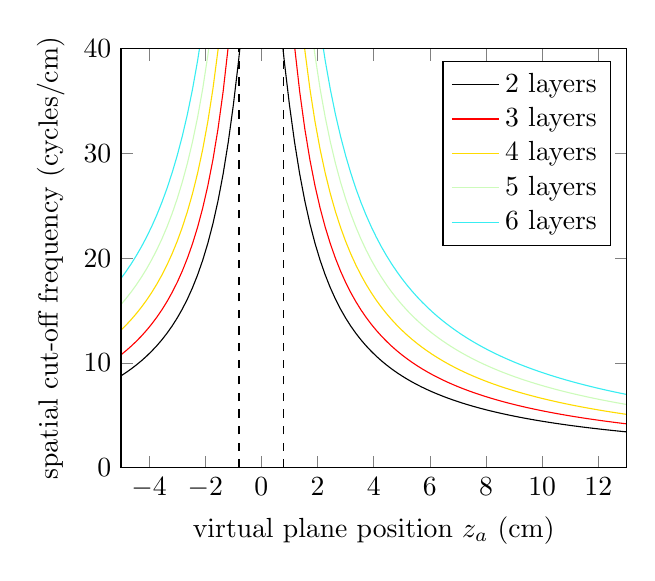
\begin{tikzpicture}
	
		\definecolor{c1}{RGB}{255, 0, 0}
		\definecolor{c2}{RGB}{255, 219, 0}
		\definecolor{c3}{RGB}{205, 251, 187}
		\definecolor{c4}{RGB}{56, 237, 242}
		\definecolor{c5}{RGB}{179, 46, 255}
	
		\pgfplotscreateplotcyclelist{mycolors}{black, c1, c2, c3, c4, c5}
		
		\begin{axis}[	legend pos = north east, 
						ymin = 0,
						ymax = 40, 
						xmin = -5,
						xmax = 13,
						domain = -5 : 13,
						xtick = {-4, -2, 0, 2, 4, 6, 8, 10, 12},
						ylabel = {spatial cut-off frequency (cycles/cm)},
						xlabel = {virtual plane position $z_a$ (cm)},
						ylabel near ticks,
						no markers,
						samples = 100, 
						cycle list name = mycolors,
						axis on top = true,
						width = 8 cm]
		
			% f_0 = 27.7 cycles/cm
			% h = 1.6 cm
		
			\addplot{2 * 27.7 * sqrt( (2 + 1) * 1.6^2 / ( (2 + 1) * 1.6^2 + 12 * (2 - 1) * (x^2) ) )};
			\addlegendentry{2 layers};
			
			\addplot{3 * 27.7 * sqrt( (3 + 1) * 1.6^2 / ( (3 + 1) * 1.6^2 + 12 * (3 - 1) * (x^2) ) )};
			\addlegendentry{3 layers};
			
			\addplot{4 * 27.7 * sqrt( (4 + 1) * 1.6^2 / ( (4 + 1) * 1.6^2 + 12 * (4 - 1) * (x^2) ) )};
			\addlegendentry{4 layers};
			
			\addplot{5 * 27.7 * sqrt( (5 + 1) * 1.6^2 / ( (5 + 1) * 1.6^2 + 12 * (5 - 1) * (x^2) ) )};
			\addlegendentry{5 layers};
			
			\addplot{6 * 27.7 * sqrt( (6 + 1) * 1.6^2 / ( (6 + 1) * 1.6^2 + 12 * (6 - 1) * (x^2) ) )};
			\addlegendentry{6 layers};
			
			\addplot[dashed] coordinates {(-0.8, 0) (-0.8, 100)};
			\addplot[dashed] coordinates {(0.8, 0) (0.8, 100)};
			 
		\end{axis}
		
	\end{tikzpicture}
\end{document}
		\caption{}
		\label{fig:cut-off-frequency_N_layers}
	\end{subfigure}%
	\caption[Spectral analysis for layered 3D displays]
			{Spectral analysis for layered 3D displays. 
			 (a) Spectral support of individual layers (red) from a display with three layers, superimposed in the same frequency domain.
				 The dashed lines mark the spatial cutoff frequency $\xi_0$.
			 (b) Combined spectral support of all three layers (gray), obtained by the convolution. 
				 The light field from figure~\ref{fig:spectral_analysis_for_light_field} can be displayed with frequencies within the region of support.
			 (c) Approximate upper bound on the depth of field for layered 3D displays with different a number of layers (\cite{WetzsteinTomo}) and constant display thickness.
				 The \emph{expected} upper bound is shown as dashed lines for two and six layers.
				 The displays extent is depicted by the dashed lines.}
	\label{fig:spectral_analysis_of_display}
\end{figure}
The sketch in figure~\ref{fig:3_layers} illustrates this for the case of three layers that are bandlimited by $\pm \xi_0$.
The three lines convolved produce a diamond shaped region of support as shown in figure~\ref{fig:3_layes_convolution}, which is the effective spectral support of the display.
This means that a light field with high frequencies outside the spectral support of the display will not be correctly displayed, or in other words, the display acts as a low-pass filter.

The \textbf{depth of field} of an automultiscopic display, as explained by~\cite{Antialiasingfor3DDisplays}, is the depth range that can be reproduced by the display in full spatial resolution.
Thus, the boundary of the spectral support describes an upper bound on the depth of field for any automultiscopic display, including layered displays.
It turns out to be quite hard to analytically derive an exact expression for the upper bound.
\cite{WetzsteinTomo} present a statistical approach and give an approximation for the upper bound on the depth of field $\lvert \xi_a \rvert$ for a plane $a$ placed at depth $z_a$ from a \mbox{$N$-layer} display with a thickness $h = z_N - z_1$:
\begin{equation}\label{eq:approx_upper_bound_spatial_cut_off}
	\lvert \xi_a \rvert \leq N \xi_0 \sqrt{ \frac{(N + 1) h^2}{(N + 1) h^2 + 12(N - 1)(z_a - Z_s)^2} }
\end{equation}
This approximation is based on the observation that the region of support approaches the shape of an ellipse when increasing the number of layers as seen in figure~\ref{fig:magnitude_response_2_3_5_layers}.
The right side of the equation is plotted in figure~\ref{fig:cut-off-frequency_N_layers} for different positions $z_a$ of the virtual plane.
\begin{figure}[tb]
	\subcaptionbox{\label{fig:spectral_support_2_layers}}{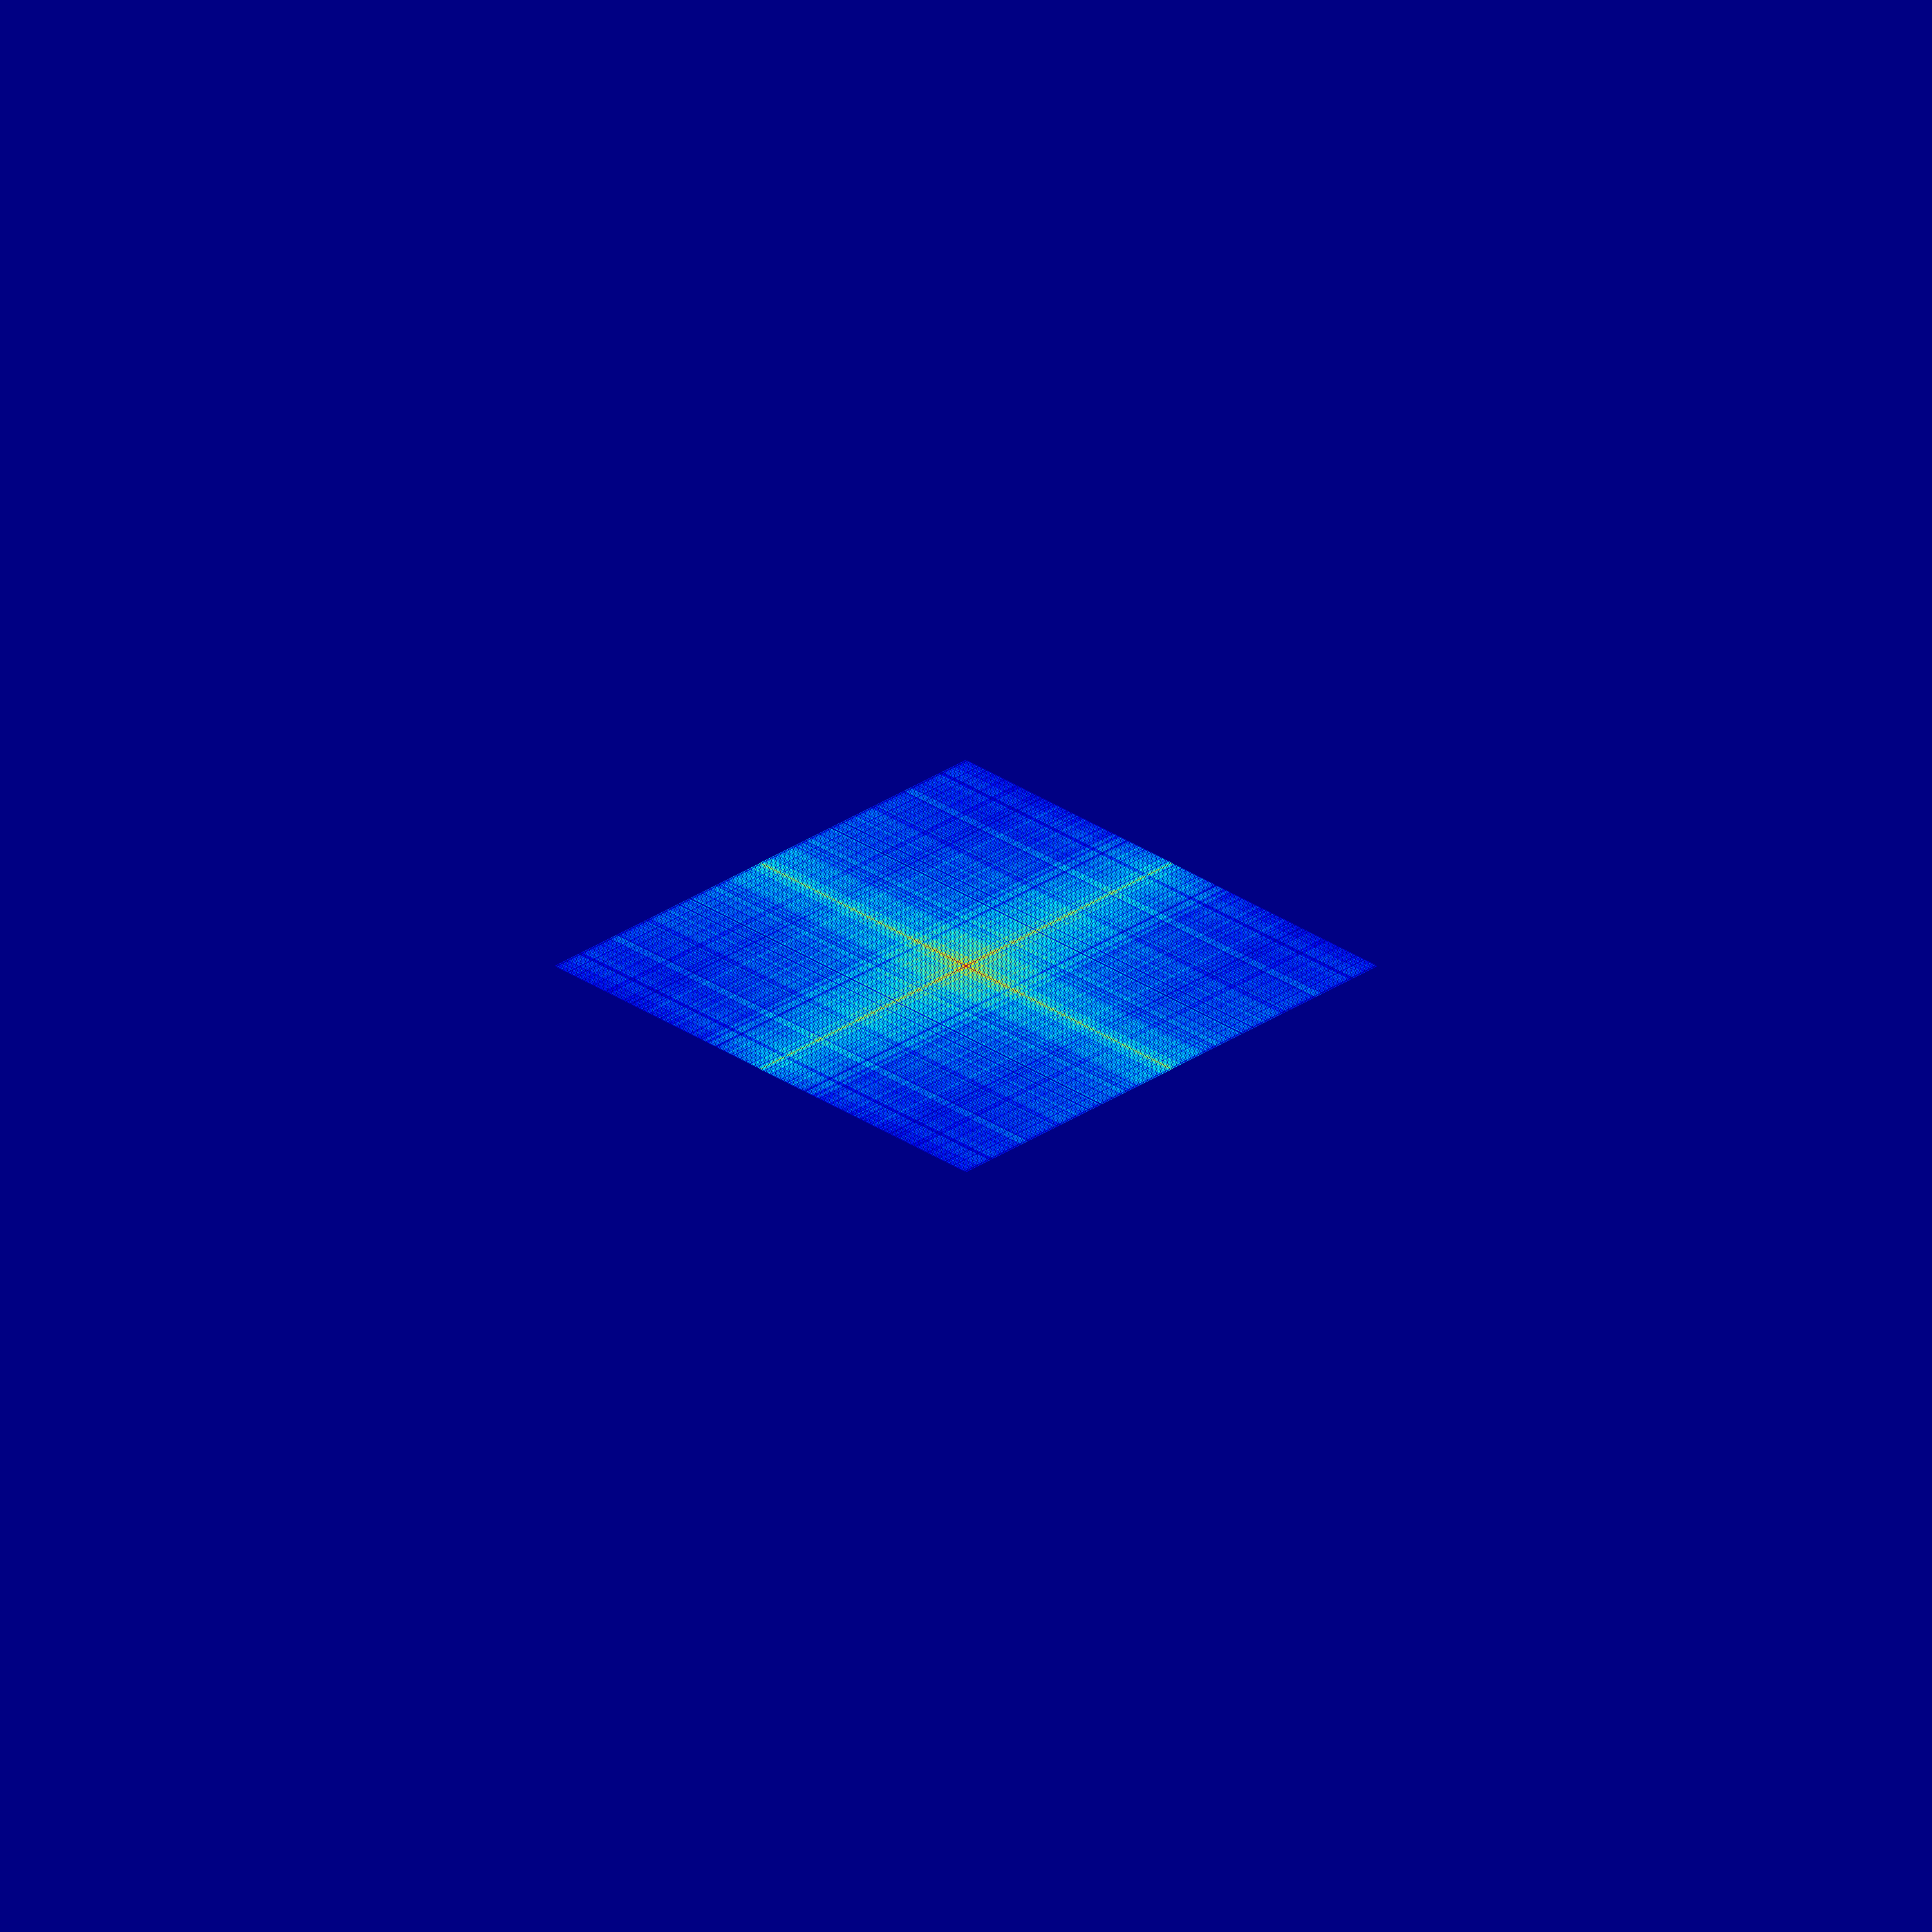
\includegraphics[height = 3.5cm]{../Figures/spectral_support/convolution_2_layers}}\hfill%
	\subcaptionbox{\label{fig:spectral_support_3_layers}}{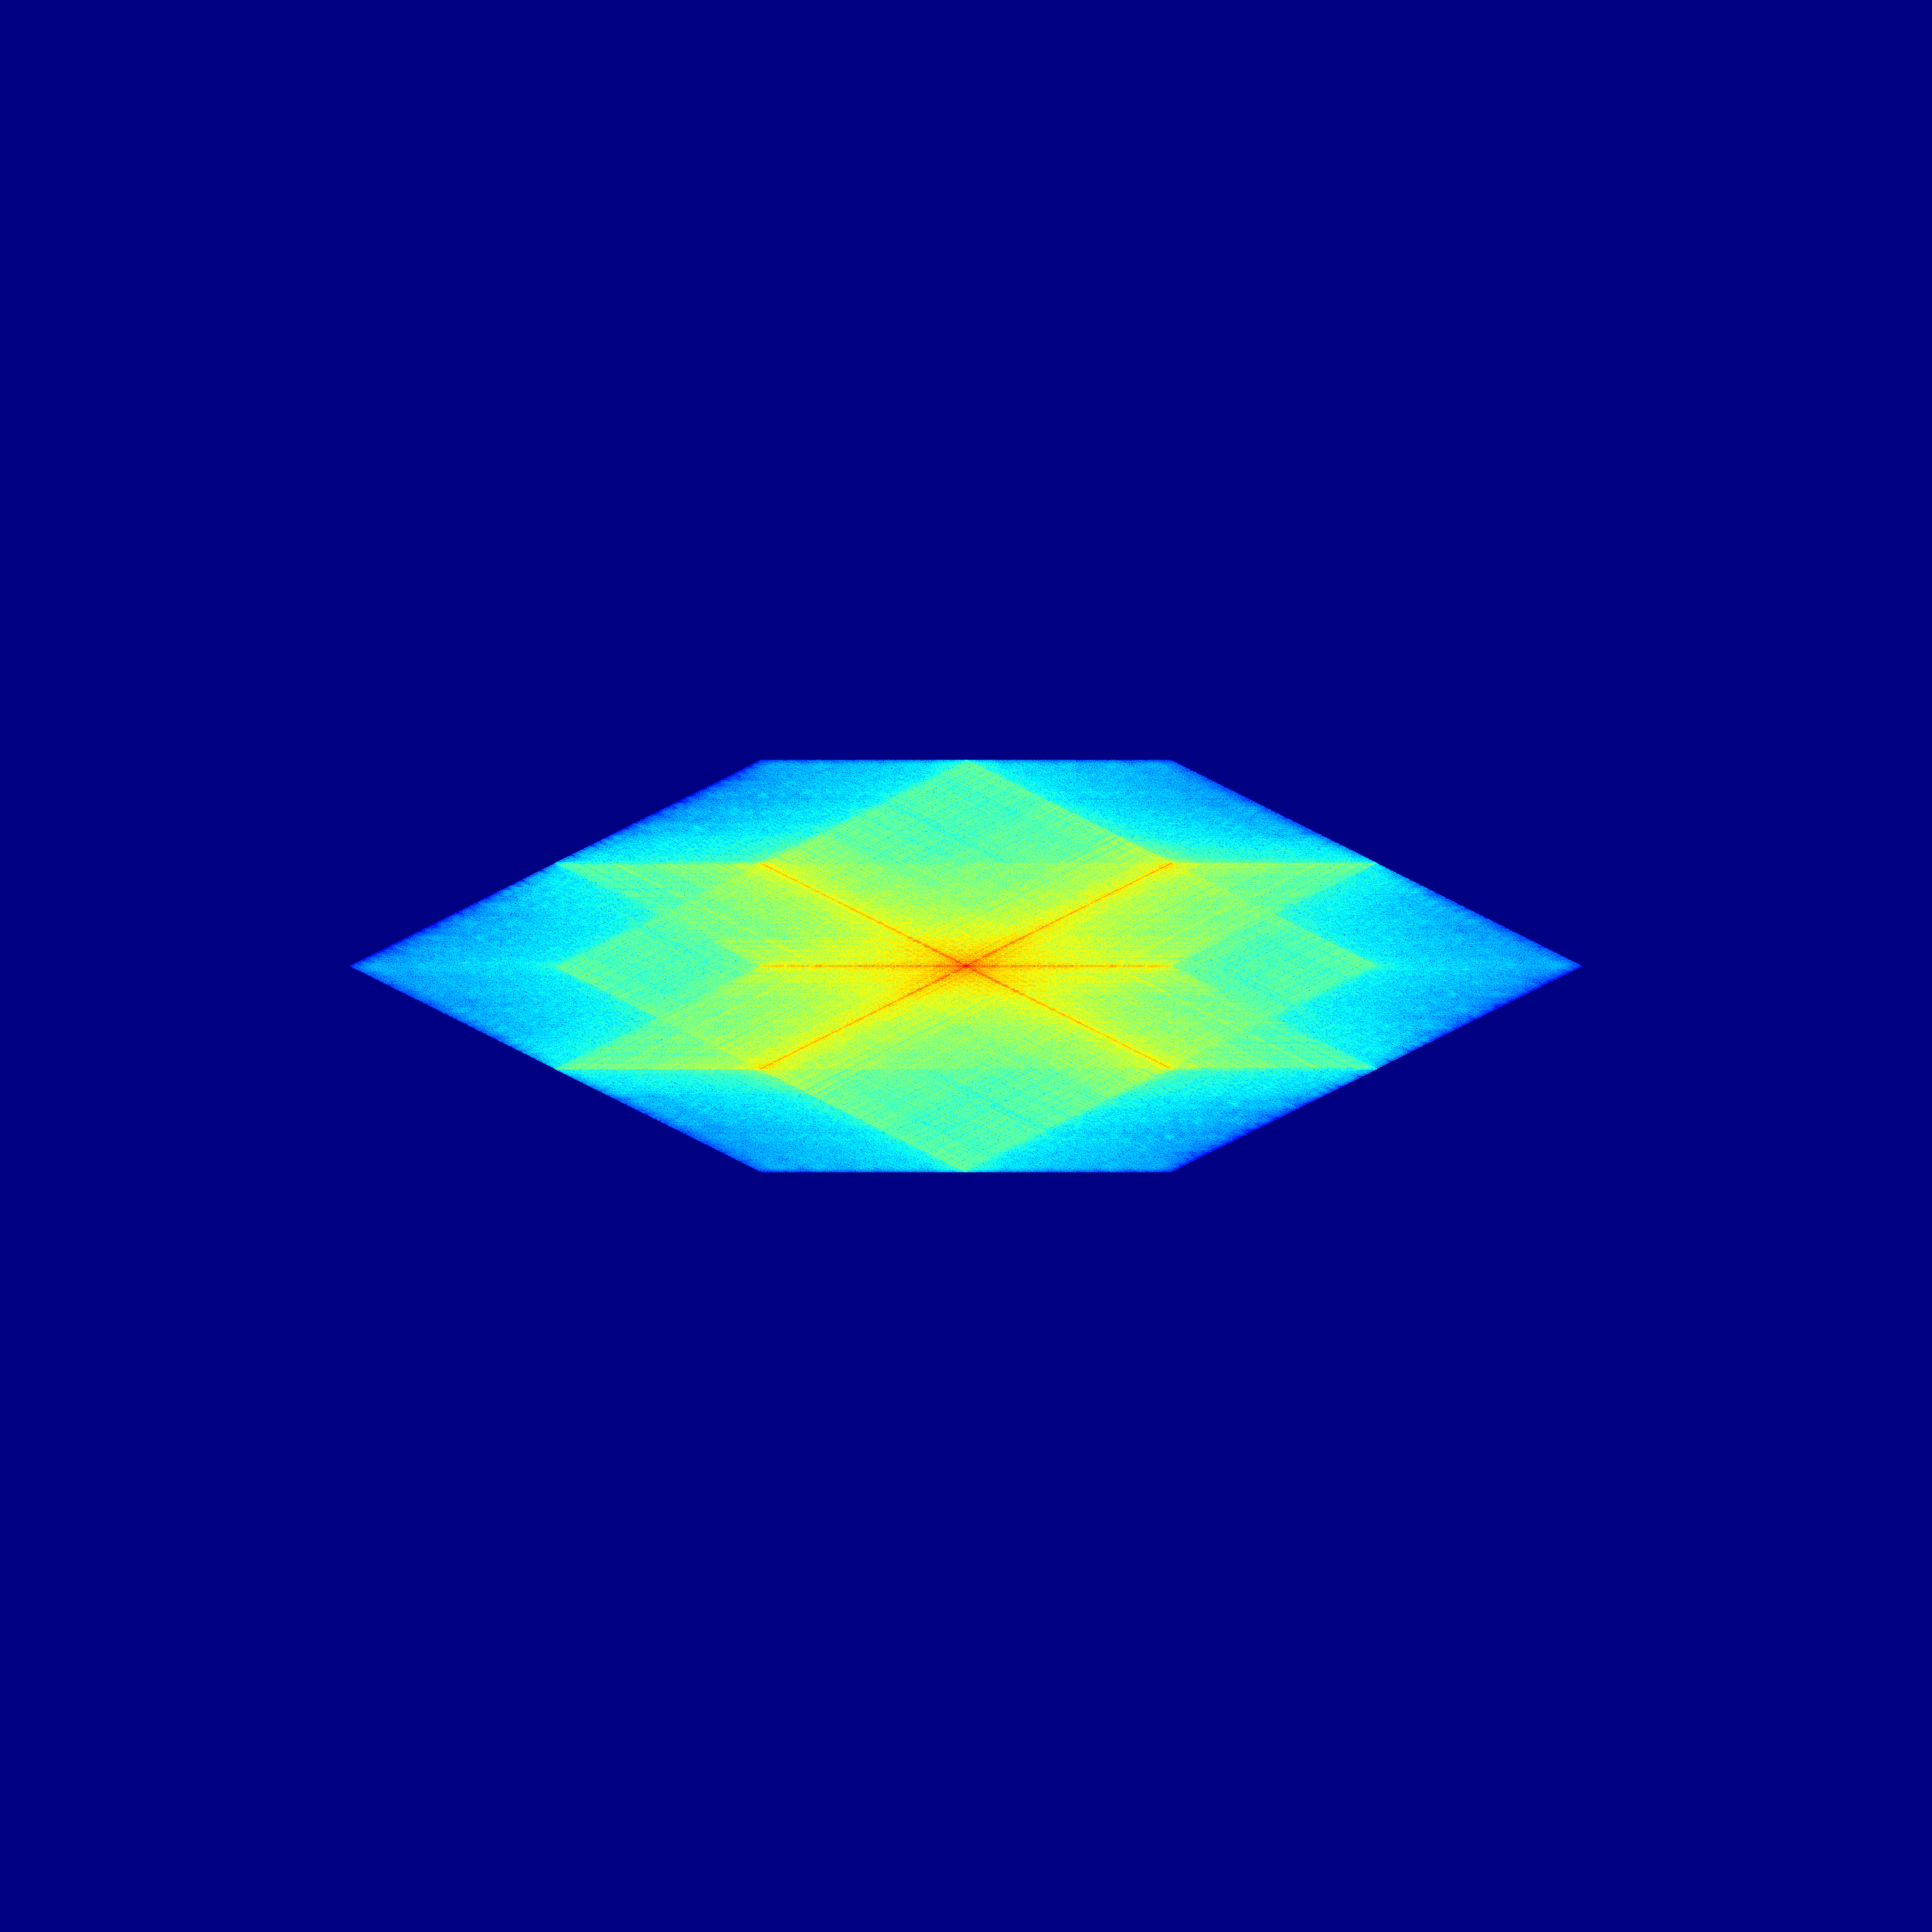
\includegraphics[height = 3.5cm]{../Figures/spectral_support/convolution_3_layers}}\hfill%
	\subcaptionbox{\label{fig:spectral_support_5_layers}}{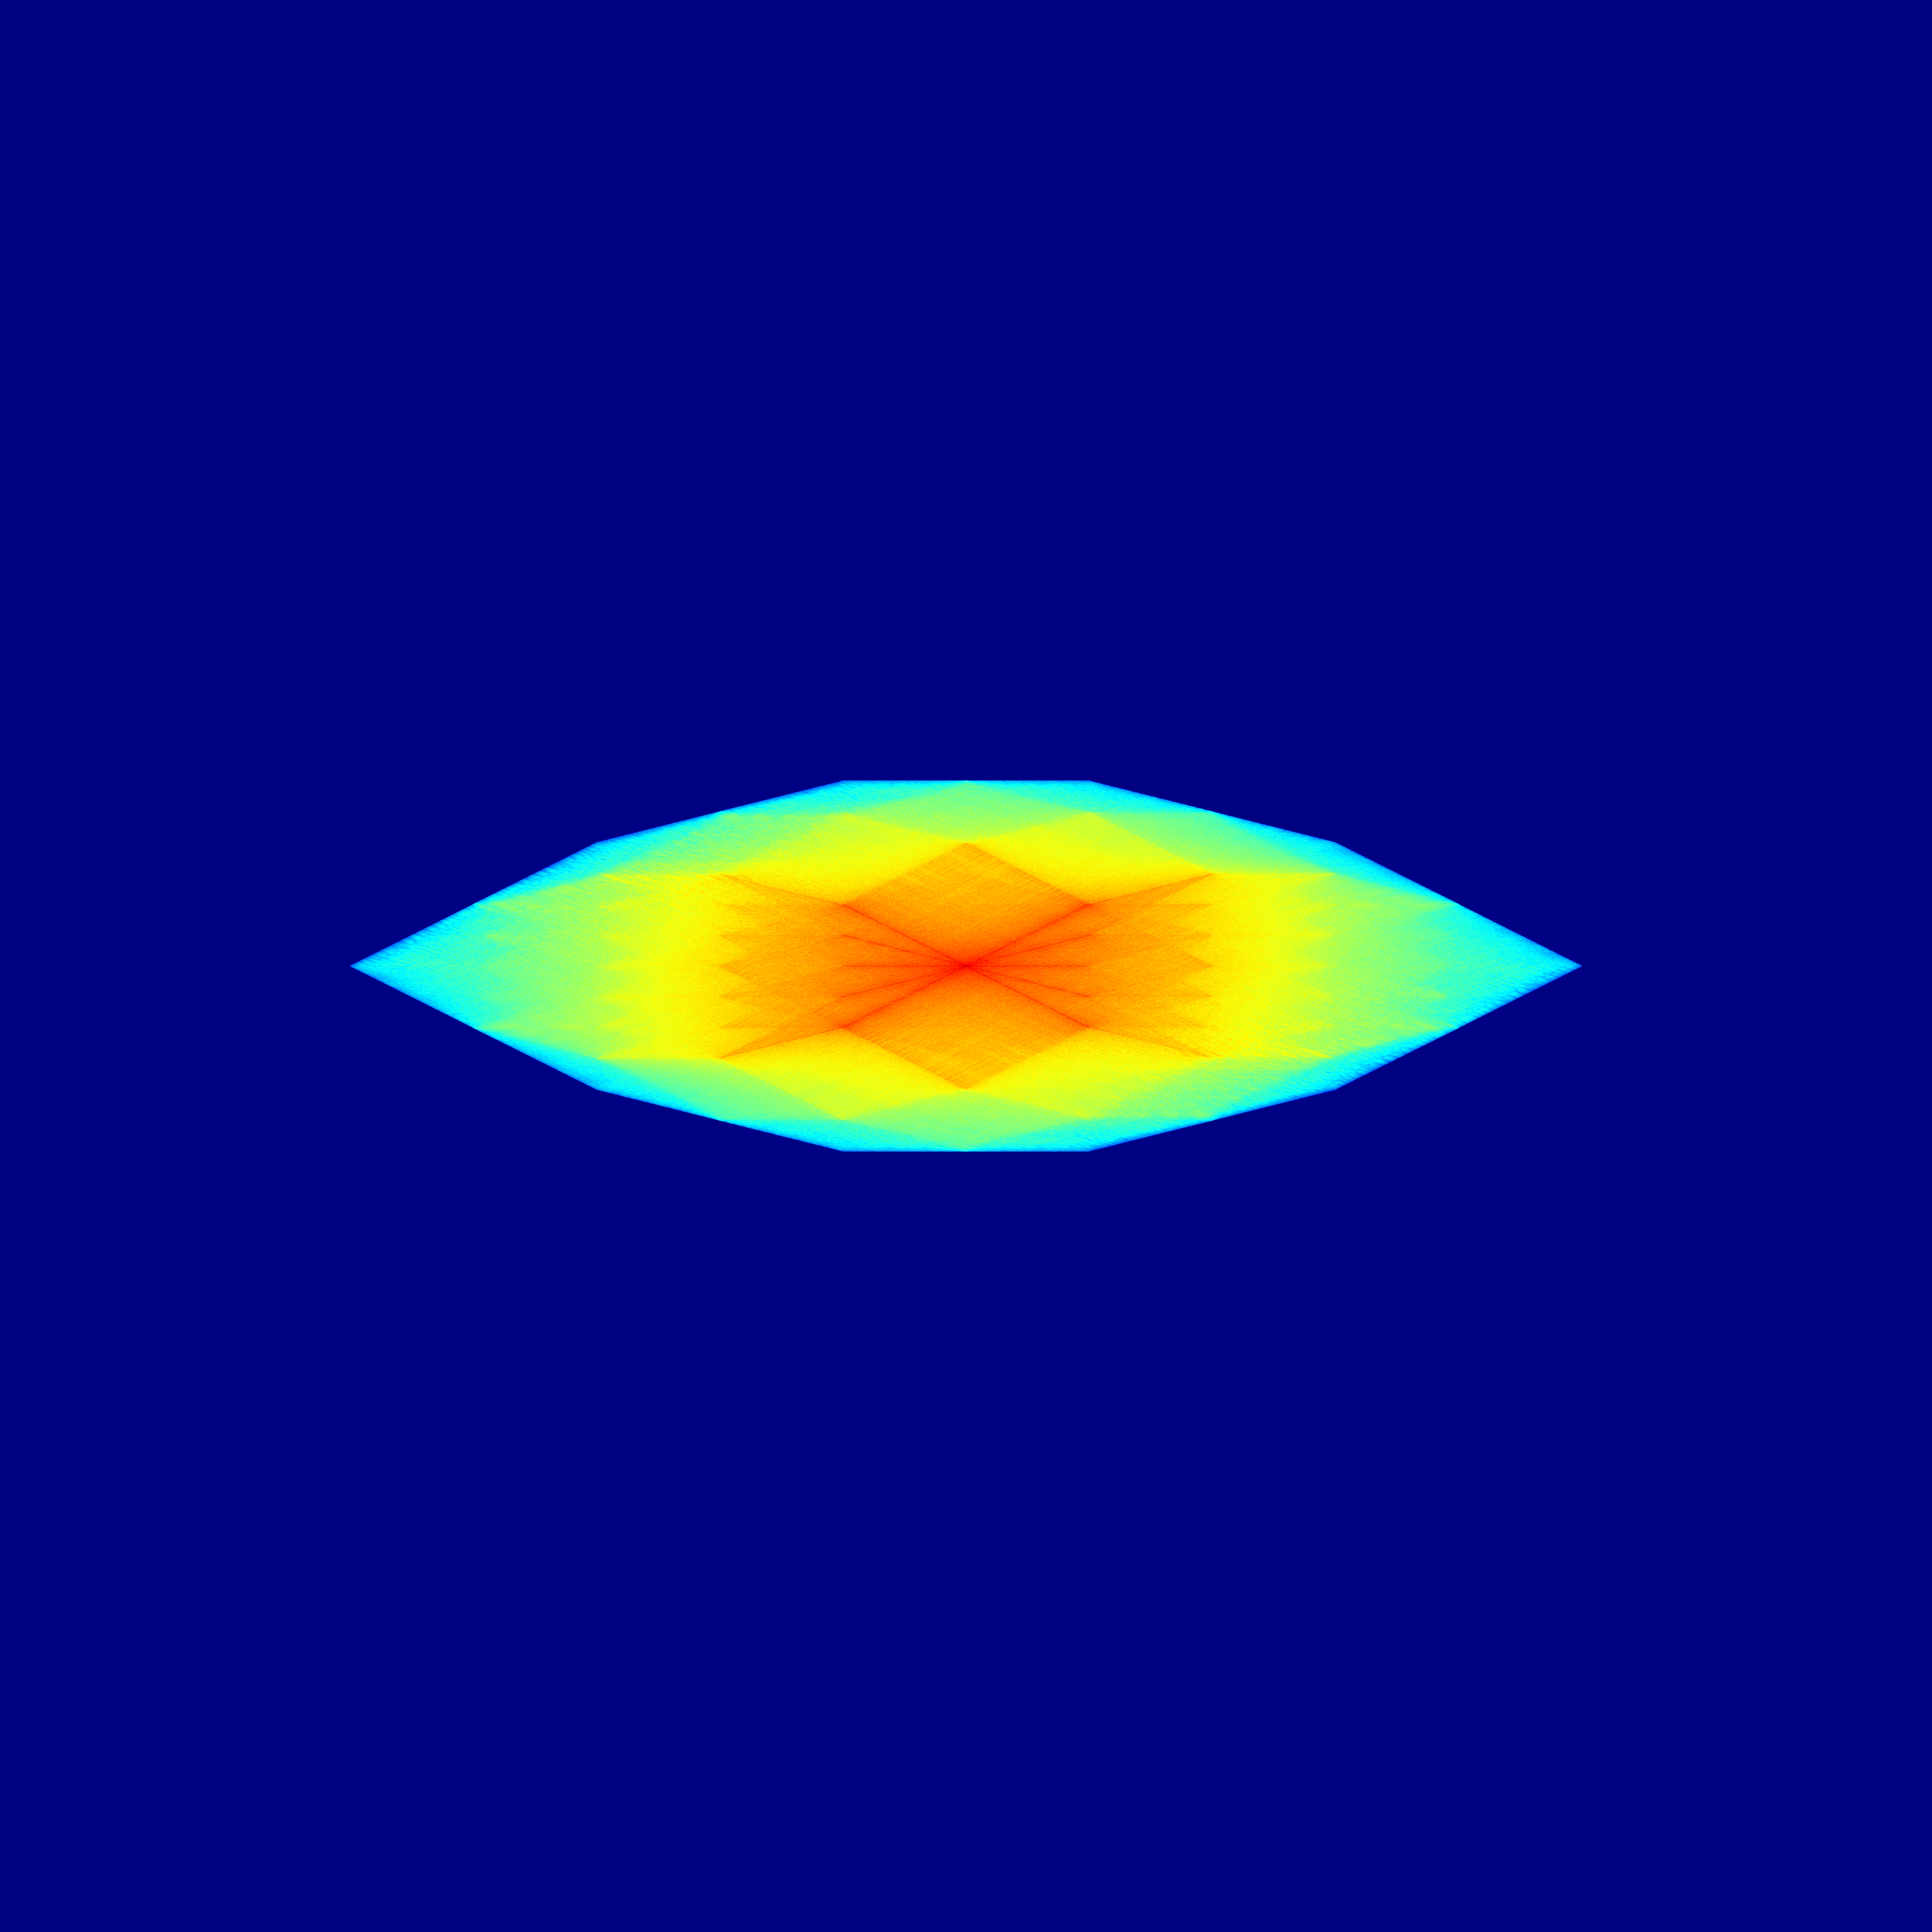
\includegraphics[height = 3.5cm]{../Figures/spectral_support/convolution_5_layers}}
	\caption[Spectral support of layered 3D displays]
			{Spectral support of layered 3D displays. 
			 The magnitude response is plotted on a logarithmic scale for a two (a), three (b) and five layer (c) display.}
	\label{fig:magnitude_response_2_3_5_layers}
\end{figure}
It shows that the spatial cut-off frequency drops rapidly when moving the virtual plane away from the display.
In fact, the drop-off is inversely proportional to $z_a$ as equation~\ref{eq:approx_upper_bound_spatial_cut_off} shows.
As figure~\ref{fig:3_layes_convolution} suggests, the display is theoretically able to produce spatial frequency that exceeds the layers cut-off $\xi_0$, even for content outside the display enclosure.
The highest spatial frequency is achieved in the middle of the display ($z_a = Z_s$), bounded by $N \xi_0$ cycles/cm as it can be deducted from equation~\ref{eq:approx_upper_bound_spatial_cut_off}.

Although this theoretical upper bound points out the limits on achievable depth of field, it is only a good reference for the ideal display and a high number of layers.
In practice, the upper bound can not be achieved in most cases due a number of reasons, including: 
Simplifications in the attenuation model, approximate solutions to equation~\ref{eq:minimize_norm} or the restriction to positive transmission values.
\cite{WetzsteinTomo} also give a more conservative expression that more closely qualifies the behavior under the mentioned restrictions:
\begin{equation}\label{eq:expected_upper_bound_spatial_cut_off}
	\lvert \xi_a \rvert \leq \xi_0 \sqrt{ \frac{2(2N - 1) h^2}{(N + 1) h^2 + 12(N - 1)(z_a - Z_s)^2} }.
\end{equation}
This is the expected upper bound on the depth of field, which is drawn as a dashed line in figure~\ref{fig:cut-off-frequency_N_layers} for a two- and six layer display.
In particular, it shows that adding more layers to the display does not necessarily increase the potential for higher depth of field.
As will be discussed in section~\ref{sec:performance_of_SART}, the addition of more layers has other benefits.